Warum sollte es nicht möglich sien die Korrektheit des Netzes mit den Vorhandenen regeln zu zeigen?

 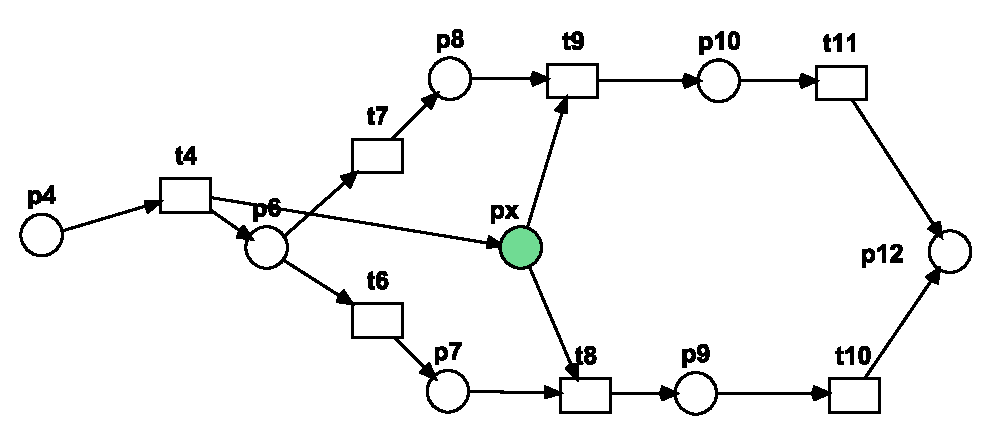
\includegraphics[scale=0.3]{Teilaufgaben/netz2.pdf}\\
 Anwenden d	er Regel P-Seq:\\
 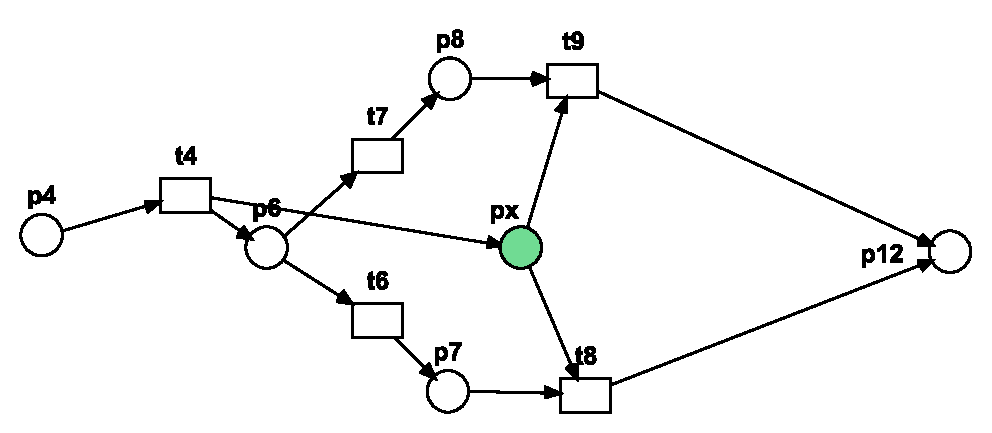
\includegraphics[scale=0.3]{Teilaufgaben/pseq1-2.pdf}\\
  Anwenden der Regel P-Seq:\\
 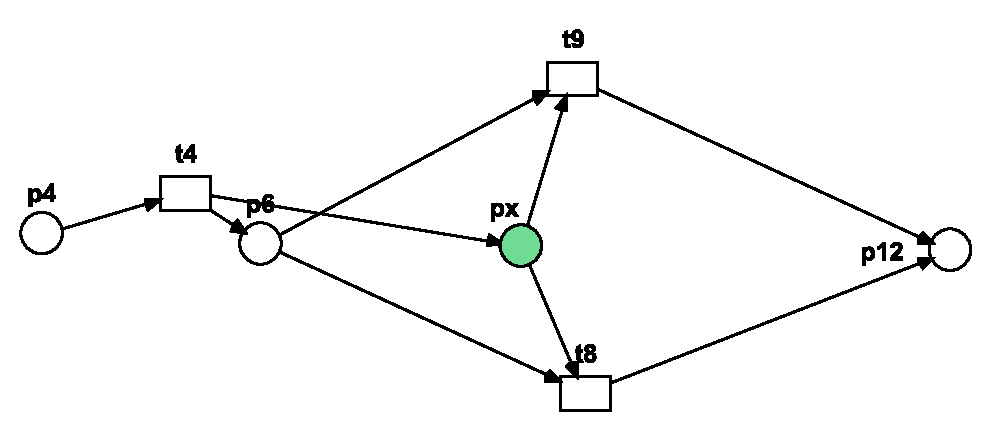
\includegraphics[scale=0.3]{Teilaufgaben/pseq2-2.pdf}\\
 
   Anwenden der Regel Same Pre/Post:\\
 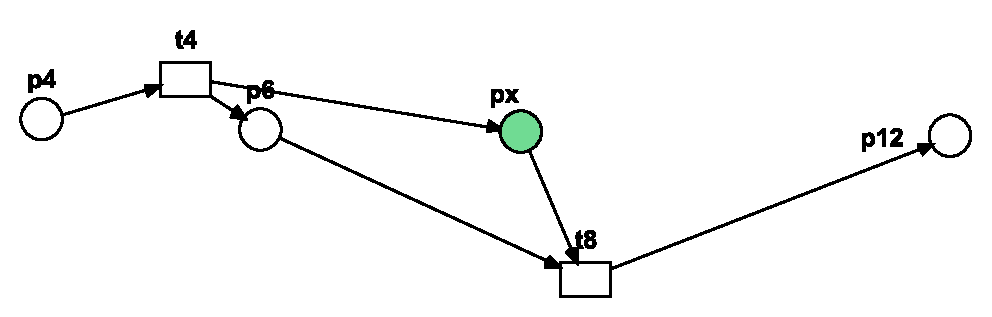
\includegraphics[scale=0.3]{Teilaufgaben/prepost1-2.pdf}\\
 
    Anwenden der Regel Par:\\
 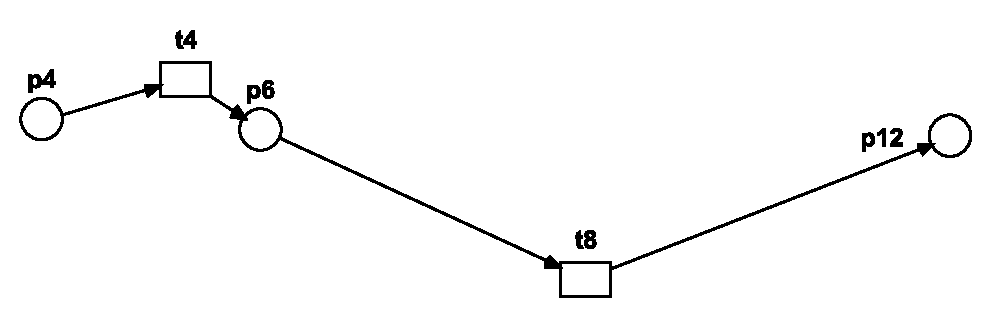
\includegraphics[scale=0.3]{Teilaufgaben/par1-2.pdf}\\
 
     Anwenden der Regel T-Seq:\\
 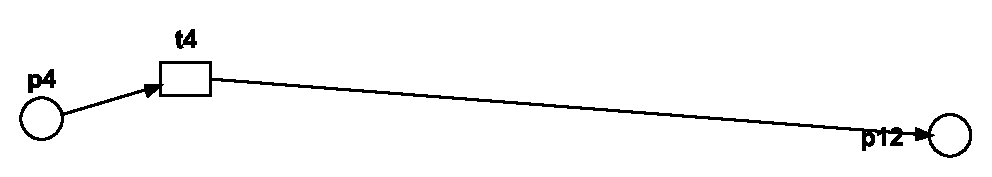
\includegraphics[scale=0.3]{Teilaufgaben/tseq1-2.pdf}\\
 
 Womit man auch auf das triviale Netz kommt.\\
 (Allerdings ist Dieses Netz Aufgrund der Fehlenden Anfangsmarkiertung sowiso Tot und damit auch nicht korrekt)